\chapter{Transcription And RNA Processing}\label{transcription-and-rna-processing}

\href{https://en.wikipedia.org/wiki/Transcription_(biology)}{Transcription} is the first of several steps of DNA based gene expression (gene is a short part of DNA that encodes for a protein), in which a particular segment of DNA is copied into RNA (especially mRNA) by the enzyme RNA polymerase. Both DNA and RNA are nucleic acids, which use base pairs of nucleotides as a complementary language. During transcription, a DNA sequence is read by an RNA polymerase, which produces a complementary, antiparallel RNA strand called a primary transcript.

Transcription proceeds in the following general steps:

\begin{enumerate}
\def\labelenumi{\arabic{enumi}.}
\tightlist
\item
  RNA polymerase, together with one or more general transcription factors, binds to promoter DNA.
\item
  RNA polymerase creates a transcription bubble, which separates the two strands of the DNA helix. This is done by breaking the hydrogen bonds between complementary DNA nucleotides.
\item
  RNA polymerase adds RNA nucleotides (which are complementary to the nucleotides of one DNA strand).
\item
  RNA sugar-phosphate backbone forms with assistance from RNA polymerase to form an RNA strand.
\item
  Hydrogen bonds of the RNA--DNA helix break, freeing the newly synthesized RNA strand.
\item
  If the cell has a nucleus, the RNA may be further processed. This may include polyadenylation, capping, and splicing.
\item
  The RNA may remain in the nucleus or exit to the cytoplasm through the nuclear pore complex.
\end{enumerate}

The stretch of DNA transcribed into an RNA molecule is called a transcription unit and encodes at least one gene. If the gene encodes a protein, the transcription produces messenger RNA (mRNA); the mRNA, in turn, serves as a template for the protein's synthesis through translation. Alternatively, the transcribed gene may encode for non-coding RNA such as microRNA, ribosomal RNA (rRNA), transfer RNA (tRNA), or enzymatic RNA molecules called ribozymes. Overall, RNA helps synthesize, regulate, and process proteins; it therefore plays a fundamental role in performing functions within a cell.

In virology, the term may also be used when referring to mRNA synthesis from an RNA molecule (i.e., RNA replication). For instance, the genome of a negative-sense single-stranded RNA (ssRNA -) virus may be template for a positive-sense single-stranded RNA (ssRNA +){[}clarification needed{]}. This is because the positive-sense strand contains the information needed to translate the viral proteins for viral replication afterwards. This process is catalyzed by a viral RNA replicase.{[}clarification needed{]}

A DNA transcription unit encoding for a protein may contain both a coding sequence, which will be translated into the protein, and regulatory sequences, which direct and regulate the synthesis of that protein. The regulatory sequence before (``upstream'' from) the coding sequence is called the five prime untranslated region (5'UTR); the sequence after (``downstream'' from) the coding sequence is called the three prime untranslated region (3'UTR).

As opposed to DNA replication, transcription results in an RNA complement that includes the nucleotide uracil (U) in all instances where thymine (T) would have occurred in a DNA complement.

Only one of the two DNA strands serve as a template for transcription. The antisense strand of DNA is read by RNA polymerase from the 3' end to the 5' end during transcription (3' → 5'). The complementary RNA is created in the opposite direction, in the 5' → 3' direction, matching the sequence of the sense strand with the exception of switching uracil for thymine. This directionality is because RNA polymerase can only add nucleotides to the 3' end of the growing mRNA chain. This use of only the 3' → 5' DNA strand eliminates the need for the Okazaki fragments that are seen in DNA replication. This also removes the need for an RNA primer to initiate RNA synthesis, as is the case in DNA replication.

The non-template (sense) strand of DNA is called the coding strand, because its sequence is the same as the newly created RNA transcript (except for the substitution of uracil for thymine). This is the strand that is used by convention when presenting a DNA sequence.

Transcription has some proofreading mechanisms, but they are fewer and less effective than the controls for copying DNA. As a result, transcription has a lower copying fidelity than DNA replication.

Transcription is divided into initiation, promoter escape, elongation, and termination.

\hypertarget{initiation-2}{%
\section{Initiation}\label{initiation-2}}

Transcription begins with the binding of RNA polymerase, together with one or more general transcription factors, to a specific DNA sequence referred to as a ``promoter'' to form an RNA polymerase-promoter ``closed complex''. In the ``closed complex'' the promoter DNA is still fully double-stranded.

RNA polymerase, assisted by one or more general transcription factors, then unwinds approximately 14 base pairs of DNA to form an RNA polymerase-promoter ``open complex''. In the ``open complex'' the promoter DNA is partly unwound and single-stranded. The exposed, single-stranded DNA is referred to as the ``transcription bubble.''

RNA polymerase, assisted by one or more general transcription factors, then selects a transcription start site in the transcription bubble, binds to an initiating NTP and an extending NTP (or a short RNA primer and an extending NTP) complementary to the transcription start site sequence, and catalyzes bond formation to yield an initial RNA product.

In bacteria, RNA polymerase holoenzyme consists of five subunits: 2 α subunits, 1 β subunit, 1 β' subunit, and 1 ω subunit. In bacteria, there is one general RNA transcription factor known as a sigma factor. RNA polymerase core enzyme binds to the bacterial general transcription (sigma) factor to form RNA polymerase holoenzyme and then binds to a promoter. (RNA polymerase is called a holoenzyme when sigma subunit is attached to the core enzyme which is consist of 2 α subunits, 1 β subunit, 1 β' subunit only).

In archaea and eukaryotes, RNA polymerase contains subunits homologous to each of the five RNA polymerase subunits in bacteria and also contains additional subunits. In archaea and eukaryotes, the functions of the bacterial general transcription factor sigma are performed by multiple general transcription factors that work together. In archaea, there are three general transcription factors: TBP, TFB, and TFE. In eukaryotes, in RNA polymerase II-dependent transcription, there are six general transcription factors: TFIIA, TFIIB (an ortholog of archaeal TFB), TFIID (a multisubunit factor in which the key subunit, TBP, is an ortholog of archaeal TBP), TFIIE (an ortholog of archaeal TFE), TFIIF, and TFIIH. The TFIID is the first component to bind to DNA due to binding of TBP, while TFIIH is the last component to be recruited. In archaea and eukaryotes, the RNA polymerase-promoter closed complex is usually referred to as the ``preinitiation complex.''

Transcription initiation is regulated by additional proteins, known as activators and repressors, and, in some cases, associated coactivators or corepressors, which modulate formation and function of the transcription initiation complex.

After the first bond is synthesized, the RNA polymerase must escape the promoter. During this time there is a tendency to release the RNA transcript and produce truncated transcripts. This is called abortive initiation, and is common for both eukaryotes and prokaryotes. Abortive initiation continues to occur until an RNA product of a threshold length of approximately 10 nucleotides is synthesized, at which point promoter escape occurs and a transcription elongation complex is formed.

Mechanistically, promoter escape occurs through DNA scrunching, providing the energy needed to break interactions between RNA polymerase holoenzyme and the promoter.

In bacteria, it was historically thought that the sigma factor is definitely released after promoter clearance occurs. This theory had been known as the obligate release model however later data showed that upon and following promoter clearance, the sigma factor is released according to a stochastic model known as the stochastic release model.

In eukaryotes, at an RNA polymerase II-dependent promoter, upon promoter clearance, TFIIH phosphorylates serine 5 on the carboxy terminal domain of RNA polymerase II, leading to the recruitment of capping enzyme (CE). The exact mechanism of how CE induces promoter clearance in eukaryotes is not yet known.

\hypertarget{elongation-2}{%
\section{Elongation}\label{elongation-2}}

One strand of the DNA, the template strand (or noncoding strand), is used as a template for RNA synthesis. As transcription proceeds, RNA polymerase traverses the template strand and uses base pairing complementarity with the DNA template to create an RNA copy (which elongates during the traversal). Although RNA polymerase traverses the template strand from 3' → 5', the coding (non-template) strand and newly formed RNA can also be used as reference points, so transcription can be described as occurring 5' → 3'. This produces an RNA molecule from 5' → 3', an exact copy of the coding strand (except that thymines are replaced with uracils, and the nucleotides are composed of a ribose (5-carbon) sugar where DNA has deoxyribose (one fewer oxygen atom) in its sugar-phosphate backbone).{[}citation needed{]}



\begin{figure}

{\centering 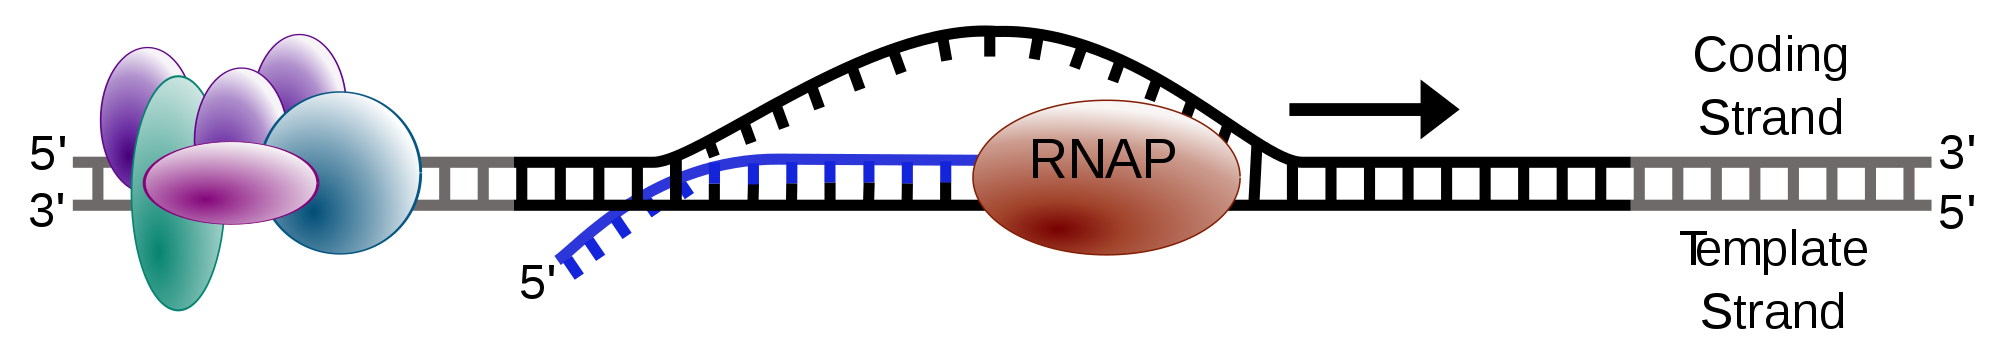
\includegraphics[width=0.7\linewidth]{./figures/transcription/Simple_transcription_elongation1} 

}

\caption{\href{https://commons.wikimedia.org/wiki/File:Simple_transcription_elongation1.svg}{RNA polymerase (RNAP) at work. Note the coding and template strands. The resulting RNA is a synthesized from the template strand and identical in sequence to the coding strand.}}\label{fig:elongation}
\end{figure}

mRNA transcription can involve multiple RNA polymerases on a single DNA template and multiple rounds of transcription (amplification of particular mRNA), so many mRNA molecules can be rapidly produced from a single copy of a gene.{[}citation needed{]} The characteristic elongation rates in prokaryotes and eukaryotes are about 10-100 nts/sec.~In eukaryotes, however, nucleosomes act as major barriers to transcribing polymerases during transcription elongation. In these organisms, the pausing induced by nucleosomes can be regulated by transcription elongation factors such as TFIIS.

Elongation also involves a proofreading mechanism that can replace incorrectly incorporated bases. In eukaryotes, this may correspond with short pauses during transcription that allow appropriate RNA editing factors to bind. These pauses may be intrinsic to the RNA polymerase or due to chromatin structure.{[}citation needed{]}

\hypertarget{termination-2}{%
\section{Termination}\label{termination-2}}

Bacteria use two different strategies for transcription termination -- Rho-independent termination and Rho-dependent termination. In Rho-independent transcription termination, RNA transcription stops when the newly synthesized RNA molecule forms a G-C-rich hairpin loop followed by a run of Us. When the hairpin forms, the mechanical stress breaks the weak rU-dA bonds, now filling the DNA--RNA hybrid. This pulls the poly-U transcript out of the active site of the RNA polymerase, terminating transcription. In the ``Rho-dependent'' type of termination, a protein factor called ``Rho'' destabilizes the interaction between the template and the mRNA, thus releasing the newl synthesized mRNA from the elongation complex.

Transcription termination in eukaryotes is less well understood than in bacteria, but involves cleavage of the new transcript followed by template-independent addition of adenines at its new 3' end, in a process called polyadenylation.

\hypertarget{inhibitors-of-transcription}{%
\section{Inhibitors of transcription}\label{inhibitors-of-transcription}}

Transcription inhibitors can be used as antibiotics against, for example, pathogenic bacteria (antibacterials) and fungi (antifungals). An example of such an antibacterial is rifampicin, which inhibits bacterial transcription of DNA into mRNA by inhibiting DNA-dependent RNA polymerase by binding its beta-subunit, while 8-hydroxyquinoline is an antifungal transcription inhibitor. The effects of histone methylation may also work to inhibit the action of transcription.

In vertebrates, the majority of gene promoters contain a CpG island with numerous CpG sites. When many of a gene's promoter CpG sites are methylated the gene becomes inhibited (silenced). Colorectal cancers typically have 3 to 6 driver mutations and 33 to 66 hitchhiker or passenger mutations. However, transcriptional inhibition (silencing) may be of more importance than mutation in causing progression to cancer. For example, in colorectal cancers about 600 to 800 genes are transcriptionally inhibited by CpG island methylation (see regulation of transcription in cancer). Transcriptional repression in cancer can also occur by other epigenetic mechanisms, such as altered expression of microRNAs. In breast cancer, transcriptional repression of BRCA1 may occur more frequently by over-expressed microRNA-182 than by hypermethylation of the BRCA1 promoter (see Low expression of BRCA1 in breast and ovarian cancers).

\hypertarget{transcription-factors}{%
\section{Transcription factors}\label{transcription-factors}}

Active transcription units are clustered in the nucleus, in discrete sites called transcription factories or euchromatin. Such sites can be visualized by allowing engaged polymerases to extend their transcripts in tagged precursors (Br-UTP or Br-U) and immuno-labeling the tagged nascent RNA. Transcription factories can also be localized using fluorescence in situ hybridization or marked by antibodies directed against polymerases. There are \textasciitilde{}10,000 factories in the nucleoplasm of a HeLa cell, among which are \textasciitilde{}8,000 polymerase II factories and \textasciitilde{}2,000 polymerase III factories. Each polymerase II factory contains \textasciitilde{}8 polymerases. As most active transcription units are associated with only one polymerase, each factory usually contains \textasciitilde{}8 different transcription units. These units might be associated through promoters and/or enhancers, with loops forming a ``cloud'' around the factor.

A molecule that allows the genetic material to be realized as a protein was first hypothesized by François Jacob and Jacques Monod. Severo Ochoa won a Nobel Prize in Physiology or Medicine in 1959 for developing a process for synthesizing RNA in vitro with polynucleotide phosphorylase, which was useful for cracking the genetic code. RNA synthesis by RNA polymerase was established in vitro by several laboratories by 1965; however, the RNA synthesized by these enzymes had properties that suggested the existence of an additional factor needed to terminate transcription correctly.{[}citation needed{]}

In 1972, Walter Fiers became the first person to actually prove the existence of the terminating enzyme.

Roger D. Kornberg won the 2006 Nobel Prize in Chemistry ``for his studies of the molecular basis of eukaryotic transcription''.

\hypertarget{rna-processing}{%
\section{RNA Processing}\label{rna-processing}}

\href{https://en.wikipedia.org/wiki/Post-transcriptional_modification}{Post-transcriptional modification} or co-transcriptional modification is a set of biological processes common to most eukaryotic cells by which an RNA primary transcript is chemically altered following transcription from a gene to produce a mature, functional RNA molecule that can then leave the nucleus and perform any of a variety of different functions in the cell. {[}1{]} There are many types of post-transcriptional modifications achieved through a diverse class of molecular mechanisms.

Perhaps the most notable example is the conversion of precursor messenger RNA transcripts into mature messenger RNA that is subsequently capable of being translated into protein. This process includes three major steps that significantly modify the chemical structure of the RNA molecule: the addition of a 5' cap, the addition of a 3' polyadenylated tail, and RNA splicing. Such processing is vital for the correct translation of eukaryotic genomes because the initial precursor mRNA produced by transcription often contains both exons (coding sequences) and introns (non-coding sequences); splicing removes the introns and links the exons directly, while the cap and tail facilitate the transport of the mRNA to a ribosome and protect it from molecular degradation.{[}2{]}

Post-transcriptional modifications may also occur during the processing of other transcripts which ultimately become transfer RNA, ribosomal RNA, or any of the other types of RNA used by the cell.

\hypertarget{mrna-processing}{%
\section{mRNA processing}\label{mrna-processing}}

The pre-mRNA molecule undergoes three main modifications. These modifications are 5' capping, 3' polyadenylation, and RNA splicing, which occur in the cell nucleus before the RNA is translated.{[}4{]}

\hypertarget{processing}{%
\subsection{5' processing}\label{processing}}

Capping of the pre-mRNA involves the addition of 7-methylguanosine (m7G) to the 5' end. To achieve this, the terminal 5' phosphate requires removal, which is done with the aid of a phosphatase enzyme. The enzyme guanosyl transferase then catalyses the reaction, which produces the diphosphate 5' end. The diphosphate 5' end then attacks the alpha phosphorus atom of a GTP molecule in order to add the guanine residue in a 5'5' triphosphate link. The enzyme (guanine-N7-)-methyltransferase (``cap MTase'') transfers a methyl group from S-adenosyl methionine to the guanine ring.{[}5{]} This type of cap, with just the (m7G) in position is called a cap 0 structure. The ribose of the adjacent nucleotide may also be methylated to give a cap 1. Methylation of nucleotides downstream of the RNA molecule produce cap 2, cap 3 structures and so on. In these cases the methyl groups are added to the 2' OH groups of the ribose sugar. The cap protects the 5' end of the primary RNA transcript from attack by ribonucleases that have specificity to the 3'5' phosphodiester bonds.{[}6{]}

\hypertarget{processing-1}{%
\subsection{3' processing}\label{processing-1}}

The pre-mRNA processing at the 3' end of the RNA molecule involves cleavage of its 3' end and then the addition of about 250 adenine residues to form a poly(A) tail. The cleavage and adenylation reactions occur primarily if a polyadenylation signal sequence (5'- AAUAAA-3') is located near the 3' end of the pre-mRNA molecule, which is followed by another sequence, which is usually (5'-CA-3') and is the site of cleavage. A GU-rich sequence is also usually present further downstream on the pre-mRNA molecule. More recently, it has been demonstrated that alternate signal sequences such as UGUA upstream off the cleavage site can also direct cleavage and polyadenylation in the absence of the AAUAAA signal. It is important to understand that these two signals are not mutually independent and often coexist. After the synthesis of the sequence elements, several multi-subunit proteins are transferred to the RNA molecule. The transfer of these sequence specific binding proteins cleavage and polyadenylation specificity factor (CPSF), Cleavage Factor I (CF I) and cleavage stimulation factor (CStF) occurs from RNA Polymerase II. The three factors bind to the sequence elements. The AAUAAA signal is directly bound by CPSF. For UGUA dependent processing sites, binding of the multi protein complex is done by Cleavage Factor I (CF I). The resultant protein complex formed contains additional cleavage factors and the enzyme Polyadenylate Polymerase (PAP). This complex cleaves the RNA between the polyadenylation sequence and the GU-rich sequence at the cleavage site marked by the (5'-CA-3') sequences. Poly(A) polymerase then adds about 200 adenine units to the new 3' end of the RNA molecule using ATP as a precursor. As the poly(A) tail is synthesised, it binds multiple copies of poly(A) binding protein, which protects the 3'end from ribonuclease digestion.{[}6{]}

\hypertarget{introns-splicing}{%
\subsection{Introns Splicing}\label{introns-splicing}}

RNA splicing is the process by which introns, regions of RNA that do not code for proteins, are removed from the pre-mRNA and the remaining exons connected to re-form a single continuous molecule. Exons are sections of mRNA which become ``expressed'' or translated into a protein. They are the coding portions of a mRNA molecule.{[}7{]} Although most RNA splicing occurs after the complete synthesis and end-capping of the pre-mRNA, transcripts with many exons can be spliced co-transcriptionally.{[}8{]} The splicing reaction is catalyzed by a large protein complex called the spliceosome assembled from proteins and small nuclear RNA molecules that recognize splice sites in the pre-mRNA sequence. Many pre-mRNAs, including those encoding antibodies, can be spliced in multiple ways to produce different mature mRNAs that encode different protein sequences. This process is known as alternative splicing, and allows production of a large variety of proteins from a limited amount of DNA.

\hypertarget{reverse-transcription}{%
\section{Reverse transcription}\label{reverse-transcription}}

Some viruses (such as HIV, the cause of AIDS), have the ability to transcribe RNA into DNA. HIV has an RNA genome that is reverse transcribed into DNA. The resulting DNA can be merged with the DNA genome of the host cell. The main enzyme responsible for synthesis of DNA from an RNA template is called reverse transcriptase.

In the case of HIV, reverse transcriptase is responsible for synthesizing a complementary DNA strand (cDNA) to the viral RNA genome. The enzyme ribonuclease H then digests the RNA strand, and reverse transcriptase synthesises a complementary strand of DNA to form a double helix DNA structure (``cDNA''). The cDNA is integrated into the host cell's genome by the enzyme integrase, which causes the host cell to generate viral proteins that reassemble into new viral particles. In HIV, subsequent to this, the host cell undergoes programmed cell death, or apoptosis of T cells. However, in other retroviruses, the host cell remains intact as the virus buds out of the cell.

Some eukaryotic cells contain an enzyme with reverse transcription activity called telomerase. Telomerase is a reverse transcriptase that lengthens the ends of linear chromosomes. Telomerase carries an RNA template from which it synthesizes a repeating sequence of DNA, or ``junk'' DNA. This repeated sequence of DNA is called a telomere and can be thought of as a ``cap'' for a chromosome. It is important because every time a linear chromosome is duplicated, it is shortened. With this ``junk'' DNA or ``cap'' at the ends of chromosomes, the shortening eliminates some of the non-essential, repeated sequence rather than the protein-encoding DNA sequence, that is farther away from the chromosome end.

Telomerase is often activated in cancer cells to enable cancer cells to duplicate their genomes indefinitely without losing important protein-coding DNA sequence. Activation of telomerase could be part of the process that allows cancer cells to become immortal. The immortalizing factor of cancer via telomere lengthening due to telomerase has been proven to occur in 90\% of all carcinogenic tumors in vivo with the remaining 10\% using an alternative telomere maintenance route called ALT or Alternative Lengthening of Telomeres.


